\documentclass[11pt]{amsart}

% Standard letter size paper with 1inch margins
\usepackage[letterpaper, margin=1in]{geometry}

% Useful packages 
\usepackage{amsmath, amssymb, amsthm, amsaddr}
\usepackage{enumerate, subcaption, graphicx, hyperref}
\usepackage{algorithm}
\usepackage{algpseudocode}
\usepackage{cite}
\usepackage{bm}

\newcommand{\I}{\mathrm{i}}
\DeclareMathOperator{\E}{e}

\title{AMATH 582: Homework 2}
\author{Hunter Lybbert} % first and last name

\address{Applied Mathematics Department, University of Washington, Seattle, WA 
\\ \texttt{hlybbert@uw.edu}}

\date{\today} % you can also just type the date instead of "\today"

\begin{document}

\maketitle

\begin{abstract}
    In this analysis of the joint movement data of OptimuS-VD we experiment with Principal Component Analysis (PCA) as a means of dimensionality reduction.
    Our goal was to build a projection of the recordings to a lower dimension than the number of coordinates, visualize the movements in this new lower dimension.
    Using the lower dimensional projection we design an algorithm that recognizes which movement OptimuS-VD is performing.
    Furthermore, we first implemented a clustering-esque classifier and evaluate it's accuracy using the training set as well as the held out test set.
    Considerations of further work are given.
\end{abstract}

\section{Introduction and Overview}\label{sec:Introduction}
There are many computationally intensive computer vision models (primarily using convolutional neural-networks) that perform well on object and movement recognition.
This was all kickstarted by a paper published in \textit{Advances in Neural Information Processing Systems} by Krizhevsky et. al.  \cite{NIPS2012_c399862d}.
In our analysis we do not make use of neural networks or deep learning, we will primarily use the Singular Value Decomposition (SVD) via PCA.
In order to understand the data and attempt to classify the movements of the robot we aimed to complete the following 5 tasks: \\
\begin{enumerate}

\item Perform PCA on our robot movement data such that PCA modes are spatial modes and coefficients are time-dependent coefficients.
Investigate how many PCA spatial modes you need to keep to approximate $X_{\rm Train}$ up to 70\%, 80\% , 90\% , 95\% in Frobenius norm (i.e., energy) and plot results. \\

\item Truncate the PCA modes set to 2 and 3 modes and plot the projected $X_{\rm Train}$ in the truncated PCA space as low dimensional 2D (PC1,PC2 coordinates) and 3D (PC1,PC2,PC3 coordinates) trajectories discuss visualization and your findings. \\

\item In order to classify each sample with type of movement establish a ground truth label for each frame from each movement sample.
Then for each movement compute its centroid (mean) in $k$-modes PCA space. \\

\item Having the ground truth, create a classifier which predicts labels each sample based on the which movement type centroid it is closest to.
Compute these predicted labels for various $k$ values of $k$-PCA truncation and report the accuracy of the trained classifier (the percentage of samples for which the ground truth and the trained labels match).
Discuss your results in terms of optimal $k$ for the classifier accuracy. \\

\item Apply this classifier to the test samples.
Report the accuracy of the classifier on the test samples.
Discuss and compare it with trained accuracy.
Try various $k$ values. \\

\item Bonus (+2 points): Implement an alternative classifier based on $k$-PCA space and compare with your
results above. \\

\end{enumerate}

In the endeavor to reduce the dimensionality of the robot movement data, classify the movements, and complete the requisite tasks, we made extensive use of several important Python packages.
Namely, Matplotlib was used to create all plots and animations \cite{Hunter:2007}.
Additionally, Scikit-learn was the primary source of using the PCA algorithm and other classification methods \cite{scikit-learn}. 
Finally, NumPy was once again a crucial tool \cite{harris2020array}.
Moreover there are important theoretical underpinnings behind the algorithm we implemented which will be cited and expounded upon in the following section.

\section{Theoretical Background}\label{sec:theory}
The primary theoretical tools we used in our analysis were the Singular Value Decomposition (SVD) of a matrix $X$ and principal component analysis (PCA) an application of the SVD.
For the purposes of this report it suffices to describe the SVD at a high level and briefly describe how it is used in PCA.
The SVD is indeed a decomposition of a matrix $A$ into 3 matrices each encapsulating information about how the matrix $A$ transforms a vector $\bm x$ when performing matrix vector multiplication such as $A \bm x$.
The decomposition is denoted as follows
\begin{equation}
A = U\Sigma V^T.
\label{eq:svd}
\end{equation}
where $U$ and $V^T$ are unitary matrices meaning they preserve magnitudes or norms and only project a vector into a new basis.
Furthermore, $\Sigma$ is a diagonal matrix with nonnegative entries on it's diagonal.
The matrix, $\Sigma$, represents the scaling that $A$ would do on the vector $\bm x$.

The diagonal entries of $\Sigma$ are ordered singular values $\sigma_1 \geq \sigma_2 \geq \sigma_3 ... \geq 0$.
In class we discussed the relationship between these singular values and the covariance matrix of $A$ if $A$ were our data of interest.
This connection leads to PCA where we use the SVD to project our data to a lower dimensional space but we preserve the dimensions with the greatest variance.
We make use of \textbf{ scikit-learn}'s PCA class, which under the hood uses \textbf{scipy}'s SVD solver.
Let's get into the actual implementation now.

\section{Algorithm Implementation and Development}\label{sec:algorithms}
The training data we were working with was provided in 15 \textit{.npy } files each containing 100 frames of the robot's 38 joint positions while performing one of three movements.
We were provided with 5 samples of each movement, \textit{walking, running, {\rm and } jumping}.
Additionally, it should be noted that the 38 joints' positions were provided in terms of 3 dimensional spatial coordinates.
So each single sample was of the shape $(114,100)$.

We want to perform PCA on the provided data using scikit-learn's implementation which expects the data input in the form of \textit{(n\_samples, n\_dimensions)}.
In order to use sklearn, we needed to decide what shape made sense for our data.
Initially I felt it made sense to reshape each of our 15 samples from $(114,100)$ to $(11400,)$ which we could stack on top of one another and then we would have a data matrix of shape $(15, 11400)$ where each row corresponds to a single sample of robot movement.
After some experimentation and consulting with classmates, the decision was made to retain the spatial dimension of 114 and to horizontally stack each of the 15 samples along the second dimension giving us a data matrix of shape $(114, 1500)$.
With this shape we can simply transpose the data and we are ready to utilize sklearn's PCA class.

As more of an exploratory step we performed an analysis of how much information or energy is retained in our data matrix given a certain number of components are retained in the PCA transformation, see Figure \ref{fig:f0} for a visualization of the percent of energy preserved by a given number of PCA components.

\begin{figure}[h]
	\centering
	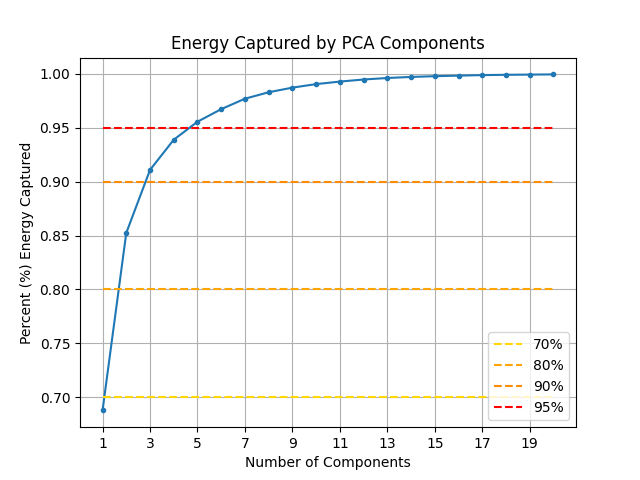
\includegraphics[width=.5\textwidth]{../visualizations/energy_by_components.png}
 	\caption{An analysis of how much information or energy is retained in our data matrix given a certain number of components are used in the PCA transformation.}\label{fig:f0}
\end{figure}

Throughout the analysis we treat each frame of each sample as a single data point which has a label and is thus classified individually as well.
We applied PCA to our compiled training data matrix twice first preserving 2 principal components and second, preserving 3 principal components.
We visualize the points projected into these lower dimensions
The projected data points (frames from the movement samples) are colored according to movement types.
See Figure \ref{fig:f1} for the visuals described.

\begin{figure}[h]
    \centering
    \begin{subfigure}{0.4\textwidth}
        \centering
        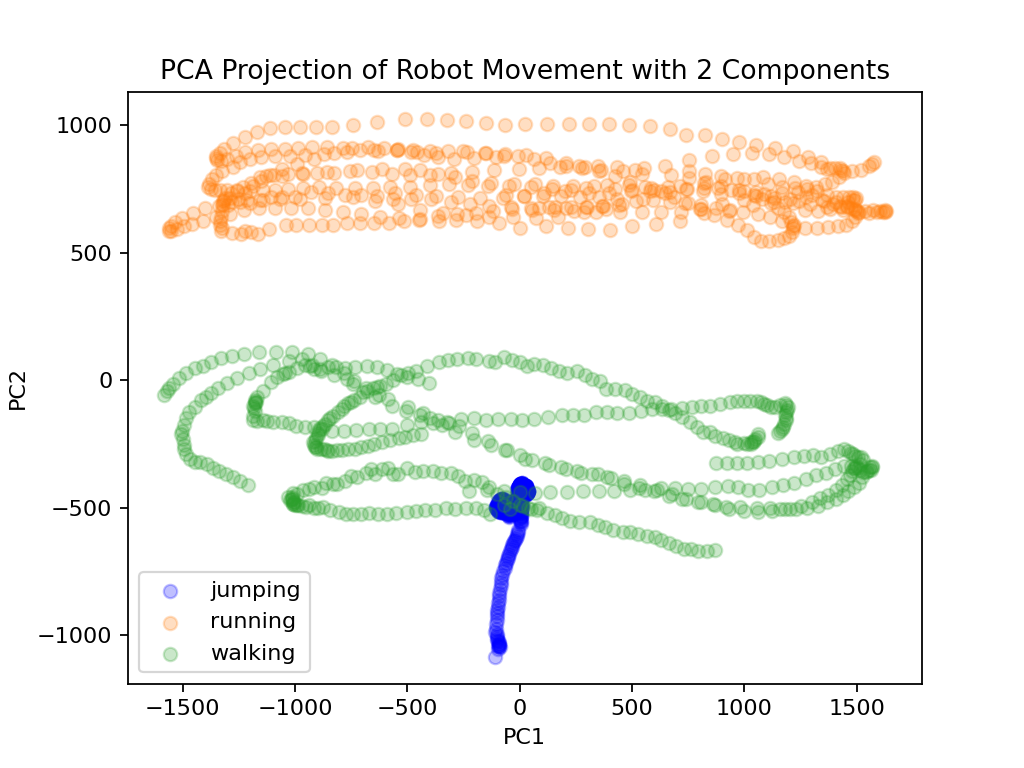
\includegraphics[width=\textwidth]{../visualizations/pca_2_components_plot.png}
        \label{fig:image1}
    \end{subfigure}
    %\hspace{1mm}
    \begin{subfigure}{0.49\textwidth}
        \centering
        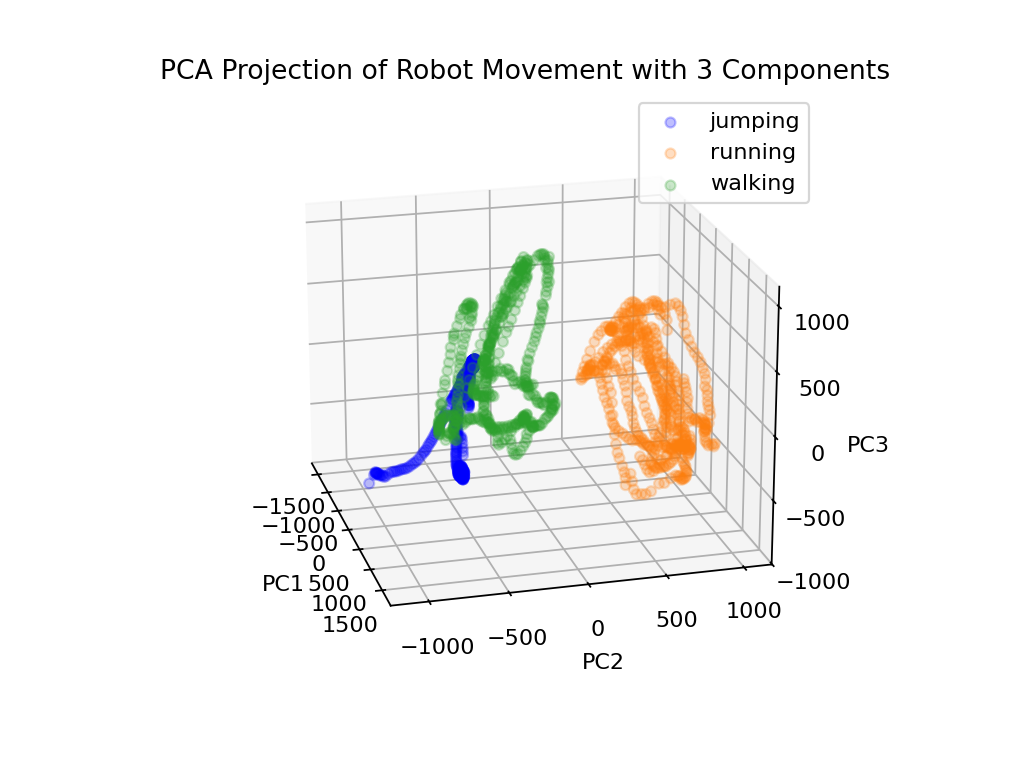
\includegraphics[width=\textwidth]{../visualizations/pca_3_components_plot.png}
        \label{fig:image2}
    \end{subfigure}
    \caption{We have visualized the lower dimensional projection of the robot movement data in both 2 and 3 dimensions.
    The projected data points (frames from the movement samples) are colored according to movement types.}
    \label{fig:f1}
\end{figure}

In order to plot according to color or to perform the next step in our algorithm, we made sure to carefully construct a ground truth array of labels which contained the corresponding movement type for each of our 1500 frames in the training data matrix of shape $(1500, 114)$ (after transposing for sklearn use).
The next step was to calculate the centroid or sample mean of the collection of frames for each movement type.
Using NumPy's builtin functionality made these centroid calculations trivial.
After calculating these centroids for each cluster of movement type, we implemented a basic classifier which classifies each point as the movement type based on which movement type's centroid it is closest to.
This was easy to implement by writing a child class inheriting from sklearn's \textbf{ClassifierMixin} and \textbf{BaseEstimator} classes.
See code for further details.
This classifier was applied to the training dataset itself as well as freshly applied to the held out test dataset to evaluate the performance of this classifier algorithm.
The findings of these evaluations will be discussed in computational results.

\section{Computational Results}\label{sec:results}
This section is only going to be a brief discussion of the results of this naive classifier based on training data centroids being calculated after PCA projections have been applied.
First and foremost, take a look at the projection and classification visualizations. Figures \ref{fig:f2} and \ref{fig:f3} are for the training set but projected to 2 and 3 dimensions respectively.
In both of these cases you can see immediately the walking and jumping clusters overlap a lot resulting in a lot of misclassification based on which centroid a given point is closest to.

\begin{figure}[h]
	\centering
	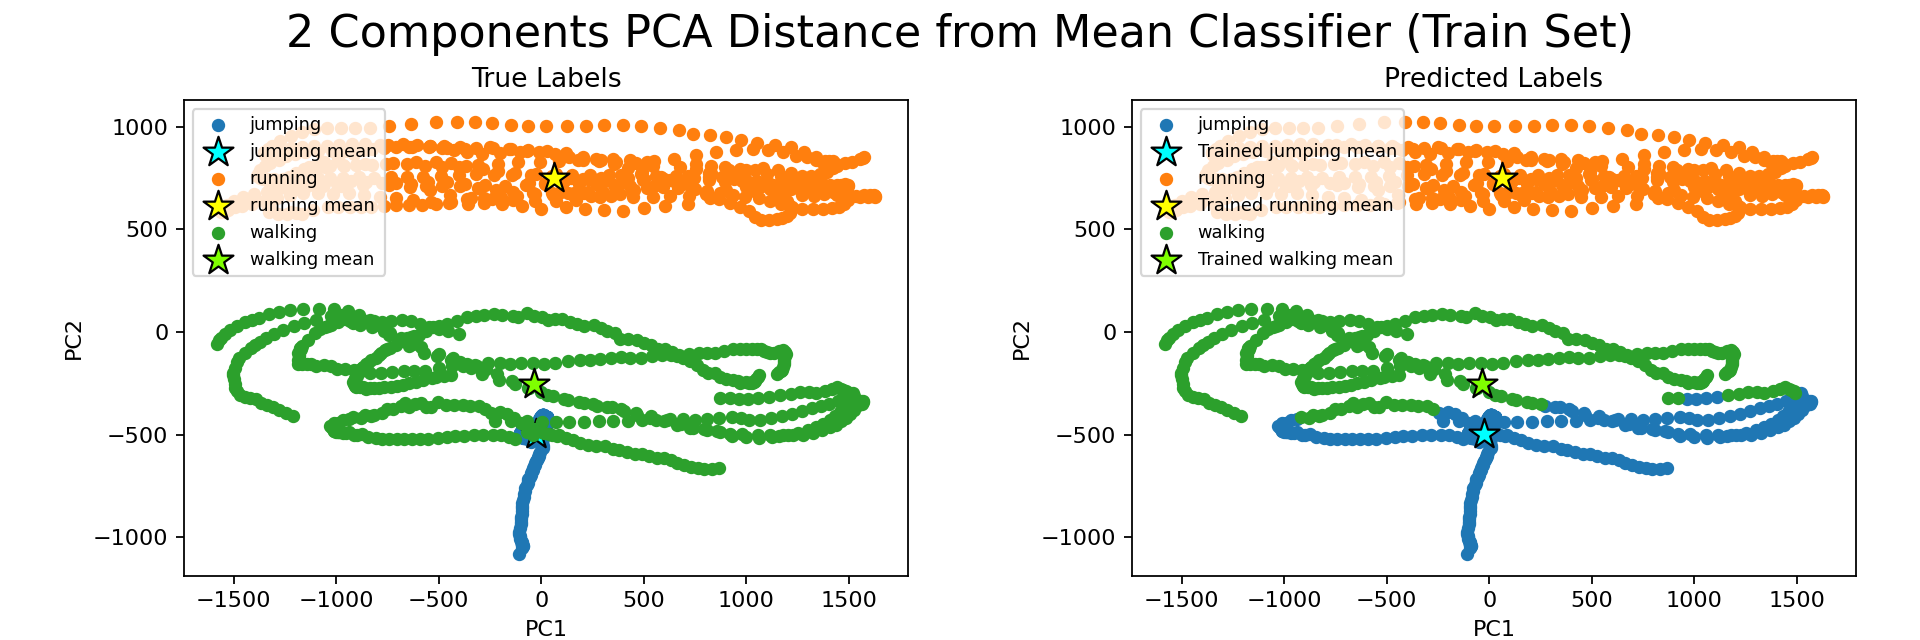
\includegraphics[width=.75\textwidth]{../visualizations/pca_distance_from_mean_classifier_2d.png}
 	\caption{On the left we are looking at the result of projecting the training set into 2 dimensions.
	The centroids we calculated have also been plotted as stars.
	Finally, on the right we have recolored each projected point by which movement type it is classified as using our centroid based classification model.}\label{fig:f2}
\end{figure}

\begin{figure}[h]
	\centering
	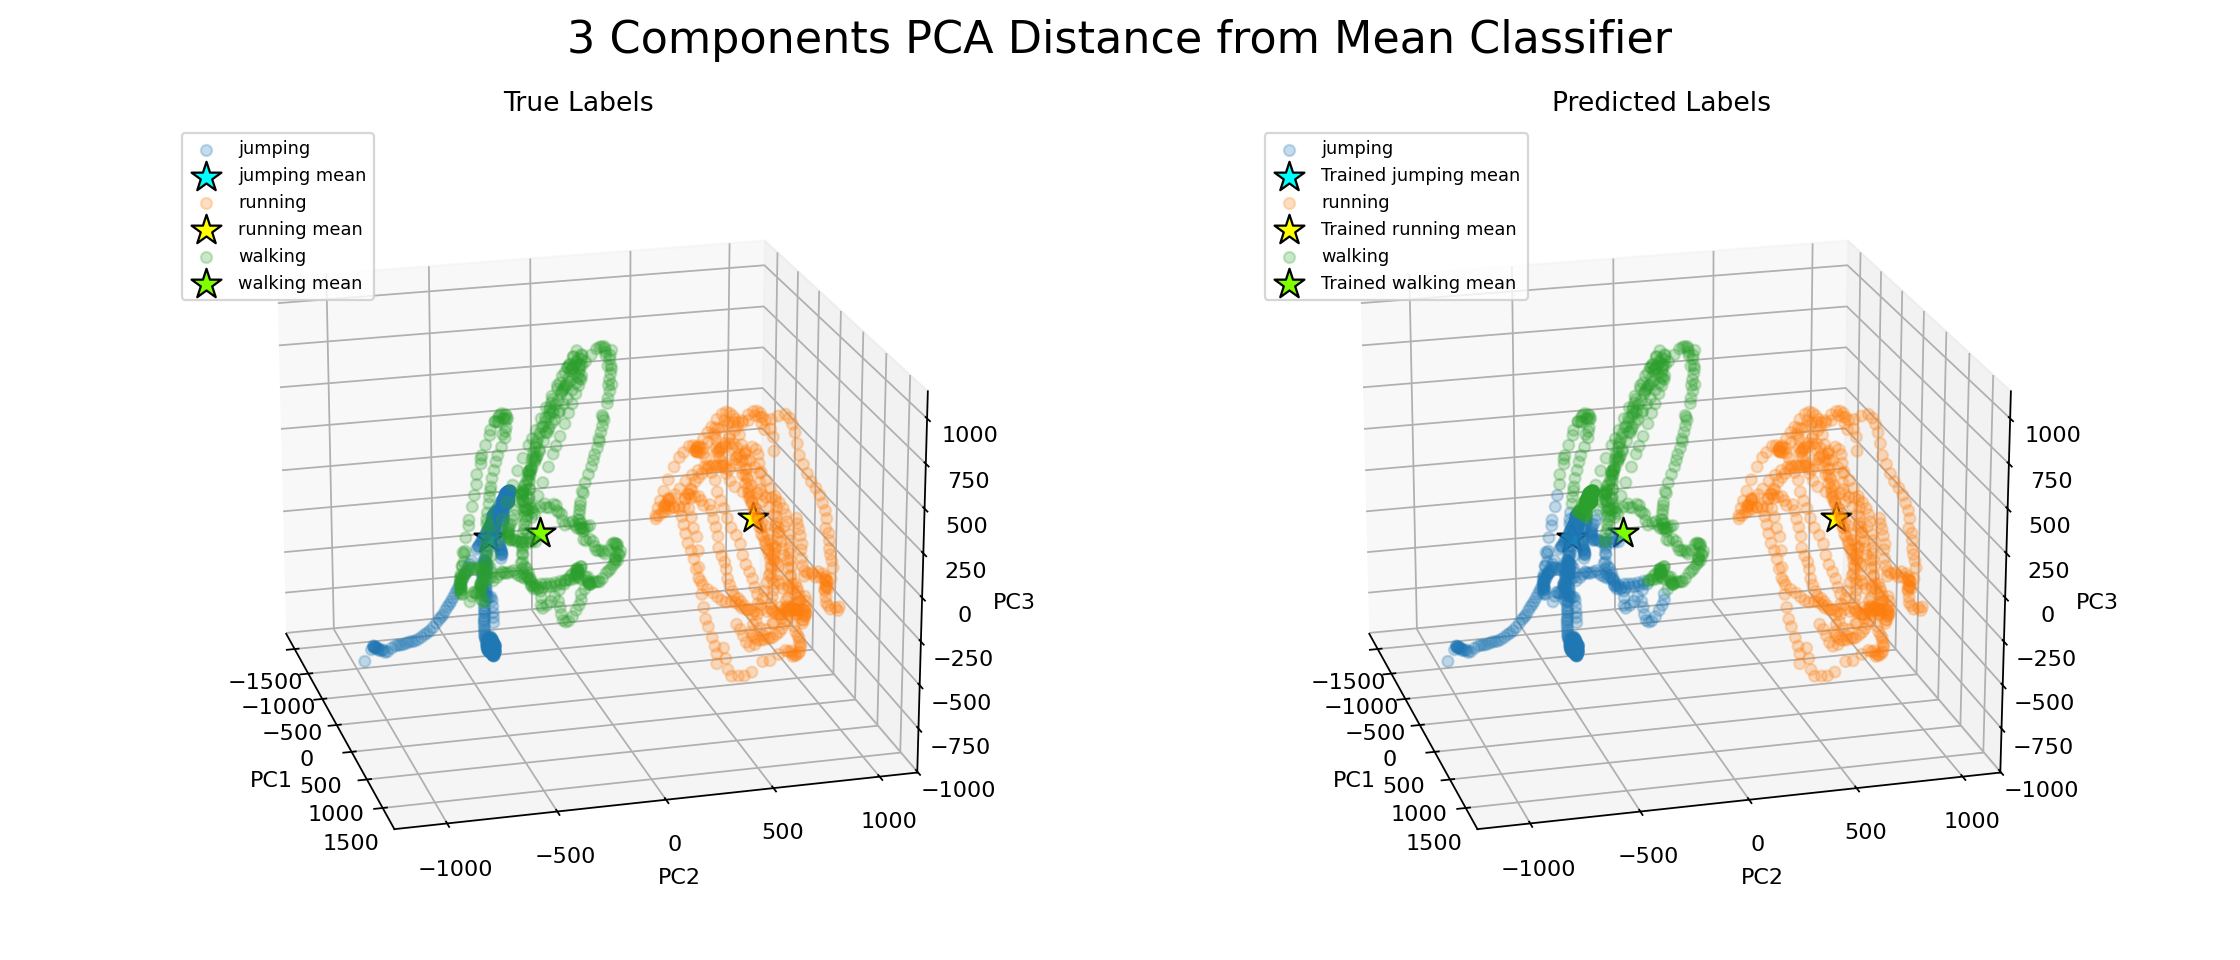
\includegraphics[width=.75\textwidth]{../visualizations/pca_distance_from_mean_classifier_3d.png}
 	\caption{This contains the same information as Figure \ref{fig:f2} with the exception that this is 3d.}\label{fig:f3}
\end{figure}

We evaluated the accuracy of this classification method on the training set for various number of components to keep when using PCA.
According to our results visualized on the left in Figure \ref{fig:f4}, the optimal number of components for accuracy would be any value of $k$ greater than 11.
However, we would likely want to choose the smallest $k$ possible since this reduces the amount of data we are storing.
So with that consideration we would choose an optimal $k$ of 11.

\begin{figure}[h]
	\centering
	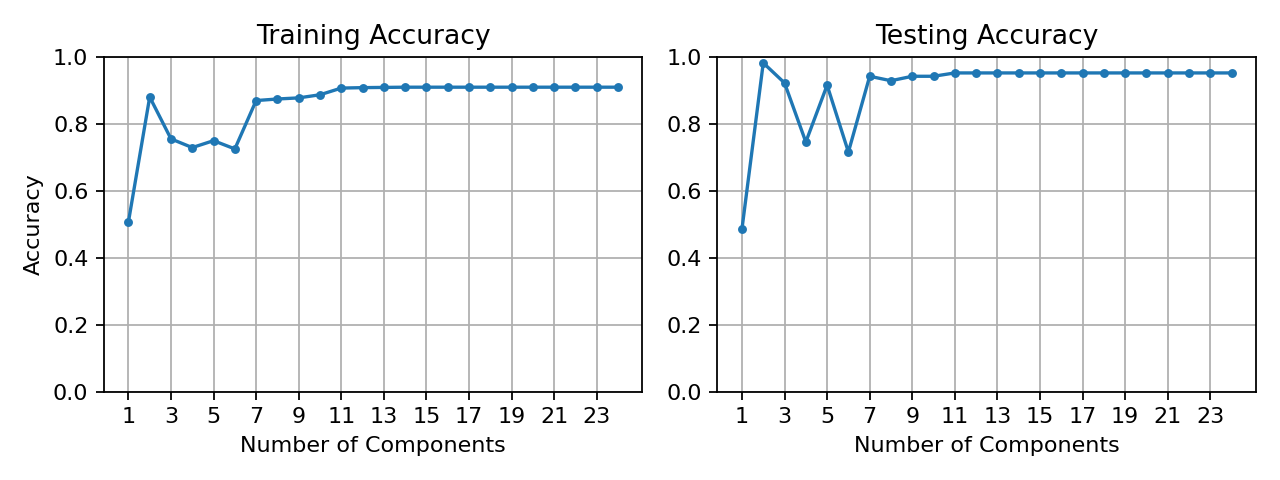
\includegraphics[width=.75\textwidth]{../visualizations/train_and_test_accuracy_by_num_components.png}
 	\caption{We performed this projection and classification for each possible number of components to keep using PCA and for both training and test sets.
	For both train and test sets we saw the level of accuracy has leveled off well before keeping only 24 components so we thought it unnecessary to plot the accuracy through all possible 114 components. }\label{fig:f4}
\end{figure}

Furthermore, we tested this method of classification on the held out test set with interesting results.
Figures \ref{fig:f5} and \ref{fig:f6} are for the training set but projected to 2 and 3 dimensions respectively.
In both of these cases we again see the walking and jumping clusters have issues.
In only 2 dimensions there are only a few miscalculated walking points interpreted to be jumping points.
This anomaly of high accuracy with only 2 components is largely due to the fact that in this dimension there is little overlap.
This could easily be an artifact of just having a small sample and perhaps getting lucky that the particular walking sample didn't intersect directly with the jumping sample in the 2d projection.

\begin{figure}[h]
	\centering
	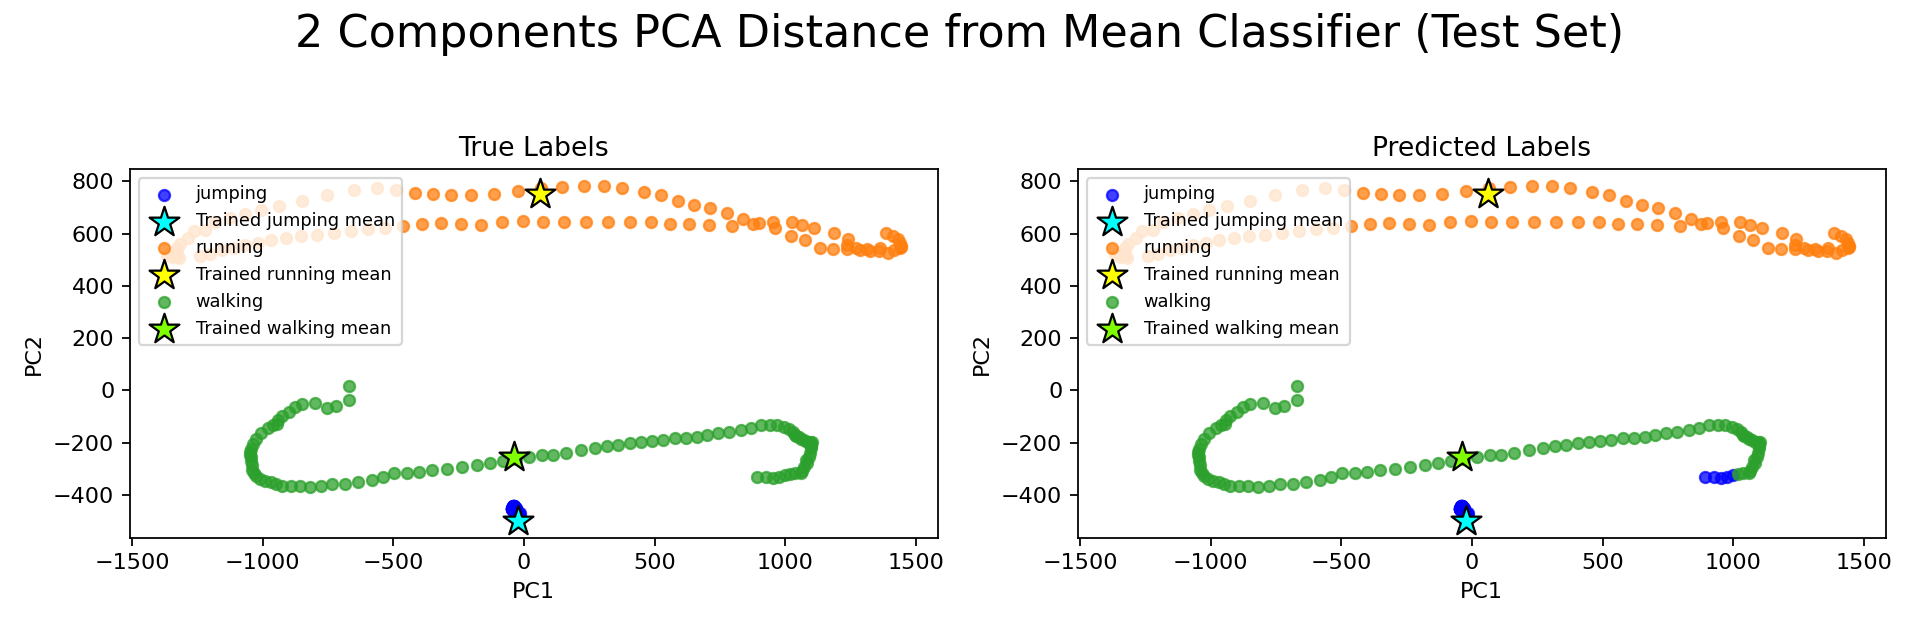
\includegraphics[width=.75\textwidth]{../visualizations/pca_distance_from_mean_classifier_2d_test_set.png}
 	\caption{On the left we are looking at the result of projecting the test set into 2 dimensions using the trained PCA projection. Additionally we have plotted the locations of the centroids as determined with the training set.
	Finally, on the right we have recolored each projected point by which movement type it is classified as using our centroid based classification model.}\label{fig:f5}
\end{figure}

\begin{figure}[h]
	\centering
	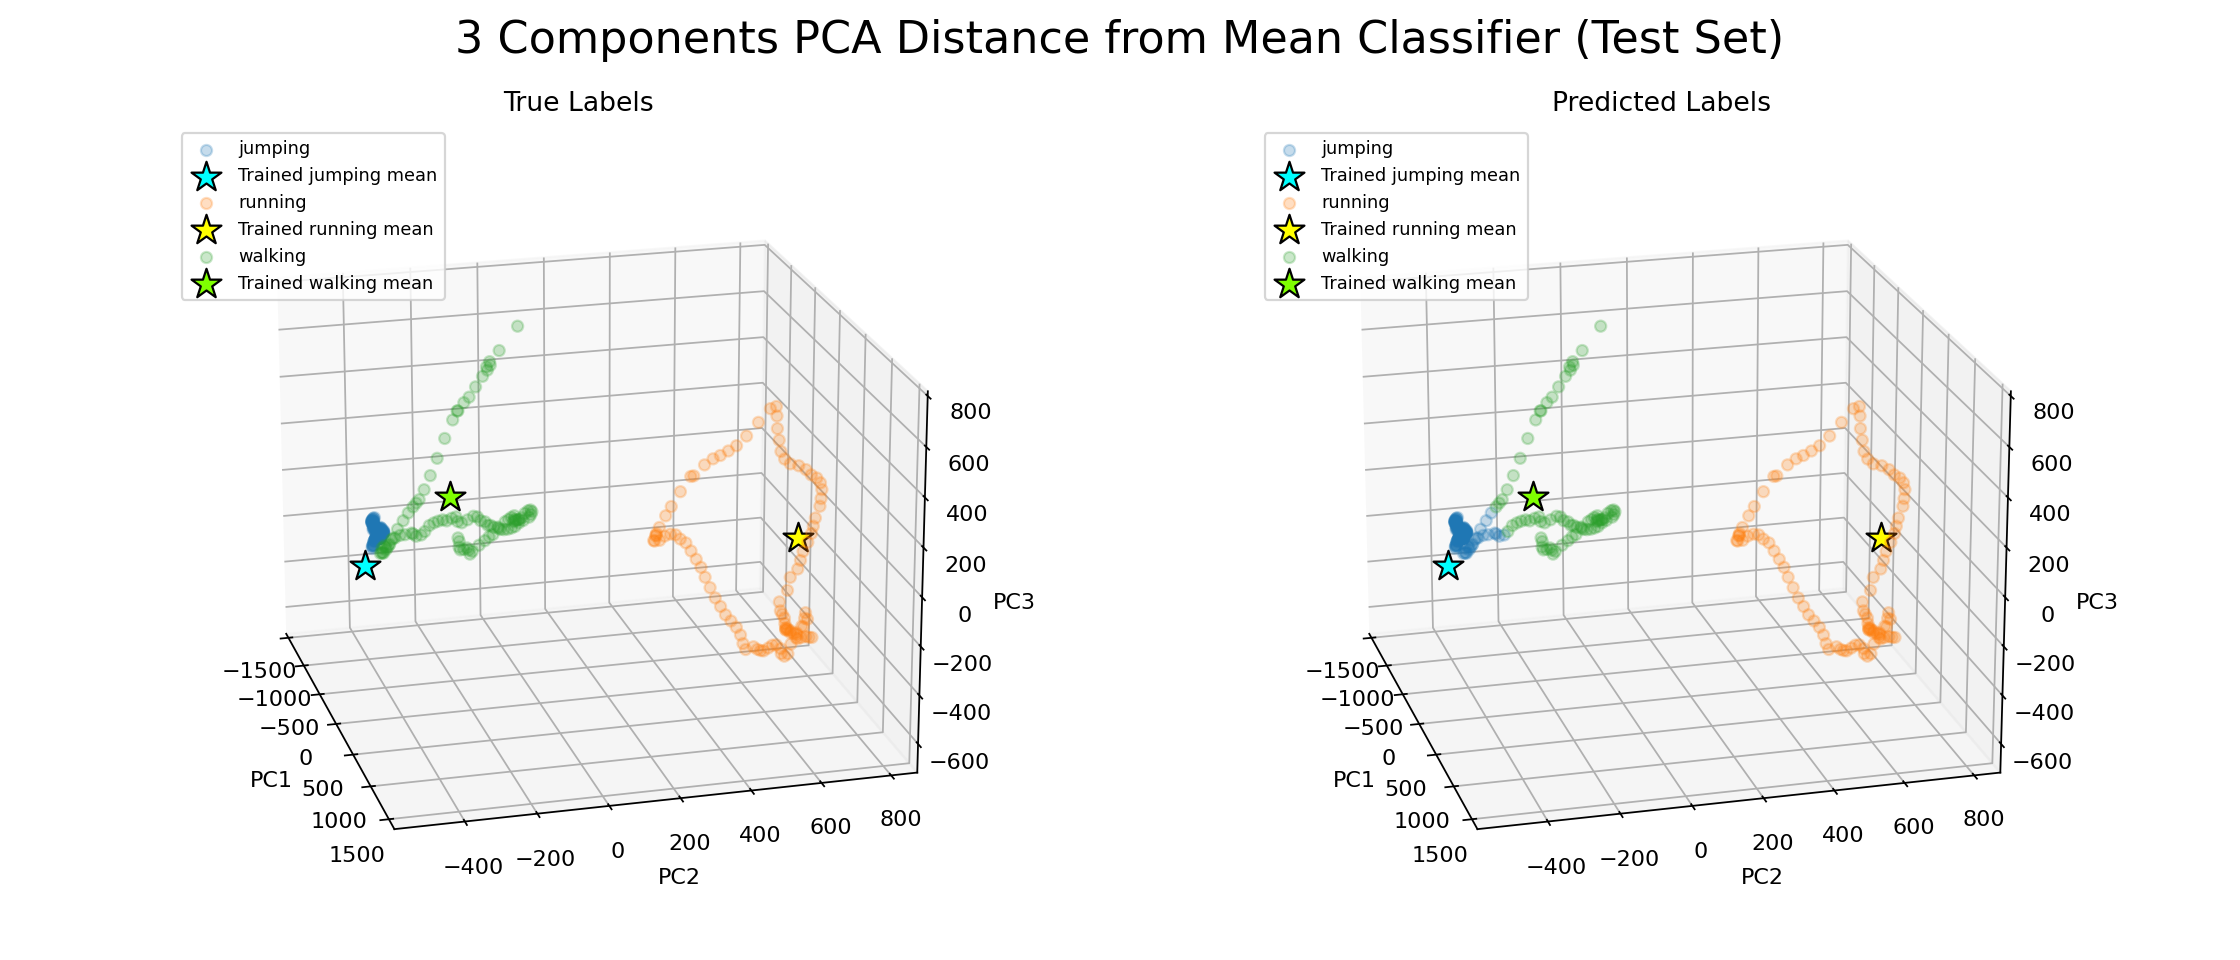
\includegraphics[width=.75\textwidth]{../visualizations/pca_distance_from_mean_classifier_3d_test_set.png}
 	\caption{This contains the same information as Figure \ref{fig:f5} with the exception that this is 3d.}\label{fig:f6}
\end{figure}

Finally, we want to acknowledge an unexpected result which we found was that the maximum accuracy score on the test set was higher than that of the training set.
We typically expect some overfitting of the training set and poor generalization which would mean high train accuracy and lower test accuracy.
Once again, I suspect that this is an artifact of only training on 15 samples and only testing on 3 samples.
This is a small training set and test set.
If we could gather more data and perform these same experiments again, we would have a better idea of what the models accuracy is like.

\section{Summary and Conclusions}\label{sec:conclusions}
Through our analysis we were able to see that some interesting structures in the data can be preserved even when reducing from 114 dimensions to 2 or 3.
We saw the reasonable results of a naive classification method and have ideas for further work.
In the future we might analyze how implementing another classifier for example a support vector machine might impact the accuracy of the model.
We would also like to try applying these methods to a larger number of samples to further expand our understanding of how these transformations and classifications generalize.

\section*{Acknowledgements} 

The author is thankful to Jaxon Tuggle for useful discussions about the process to find the correct dimensions to use when interpreting the training data samples we were given.
We would also like to thank Professor Eli Shlizerman for carefully instructing us in class.
Finally, it is necessary to thank the following students Nate Ward, Sophie Kamien, Anja Vogt, John Murphy, and Hailey Sparks whose questions helped clarify understanding of the algorithm we implemented by giving chances to explain ideas and debug code together.

\bibliographystyle{abbrv}
\bibliography{references_hw2} % make sure this matches the .bib file for your corresponding document. You also have to maintain your references in the .bib file 

\end{document}
